%!TEX root = etdrtemplate.tex
% +--------------------------------------------------------------------+
% | Sample Chapter 2
% +--------------------------------------------------------------------+

\cleardoublepage

% +--------------------------------------------------------------------+
% | Replace "This is Chapter 2" below with the title of your chapter.
% | LaTeX will automatically number the chapters.
% +--------------------------------------------------------------------+

\chapter{Background}
\label{background}

This chapter is brief introduction of all technologies and tools used in this thesis. It is SPARK/Ada programming language and its tools (GNAT Programming Studio, Sireum Bakar, GNATprove), AADL modeling language, BLESS (AADL annex language). There is also overview of the context in which this work has been made: Integrated Clinical Environment standard (ICE) and PCA Pump (ICE compliant device). This is followed by main topic of the thesis: code generation from AADL and analysis of existing AADL translators (Ocarina, RAMSES).



\section{Integrated Clinical Environment}
\label{background:ice}
Medical devices are safety-critical systems.
http://santos.cis.ksu.edu/MDCF/doc/ICE-Motivation.pdf
http://santos.cis.ksu.edu/MDCF/doc/MDCF-Tutorial-Overview.pdf
MDCF conforms to ICE standards. Medical Devices, which are ICE compliant can be connected to MDCF. It enable many Medical Devices cooperation.



\section{AADL}
\label{background:aadl}

AADL stands for Architecture Analysis \& Design Language. The aim of the AADL is to allow the description of Distributed Real-Time Embedded (DRE) systems by assembling separately developed blocks. Thus it focuses on the definition of clear block interfaces, and separates the implementations from those interfaces. AADL allows for the description of both software and hardware parts of a system \footnote{http://penelope.enst.fr/aadl}.

AADL is a language for Model-Based Engineering \cite{AadlBook}.
%https://wiki.sei.cmu.edu/aadl/index.php/The_Story_of_AADL

\subsection{Osate}
\label{background:aadl:osate}
OSATE is a set of plug-ins on top of the open-source Eclipse platform to provide a toolset for front-end processing of AADL models. It is developed mainly by SEI (Software Engineering Institute - CMU). %http://www.aadl.info/aadl/currentsite/tool/osate.html



\section{BLESS}
\label{background:bless}
How it fits into the picture. Why it was developed. Corectness prove in AADL + behavior \cite{Bless:Paper}, from which we can generate SPARK/Ada code.



\section{SPARK/Ada}
\label{background:spark}

First version of Ada programming language, Ada 83 was designed to meet the US Department of Defence Requirements formalized in "Steelman" document \footnote{http://www.adahome.com/History/Steelman/steelman.htm}. Since that time, Ada evolved. There were Ada 95, Ada 2005 and now we have Ada 2012 (released in December 10, 2012) \footnote{http://www.ada2012.org}. Ada is activelly used in many Real-World projects, e.g. Aviation, Railway Transportation, Commercial Rockets, Satellites and even Banking \cite{AdaUsaege:Online}.

SPARK is a programming language and static verification technology designed specifically for the development of high integrity software. First designed over 20 years ago, SPARK has established a track record of use in embedded and critical systems across a diverse range of industrial domains where safety and security are paramount \cite{Barnes:Book}. 

SPARK provides a significant degree of automation in proving exception freedom \cite{Spark:Article}. SPARK excludes some Ada constructs to make static analysis feasible \cite{Spark:Article}. First version of SPARK was based on Ada 83. SPARK 2005 is based on Ada 2005. It includes annotation language that support flow analysis and formal verification. Annotations are encoded in Ada comments (via the prefix \lstinline[basicstyle=\ttfamily]{--#}). It makes every SPARK 2005 programm, valid Ada 2005 program.

\begin{lstlisting}[language=ada, frame=single, gobble=0, caption={SPARK 2005 code: Odometer \cite{Barnes:Book}}]
	package Odometer
	--# own Trip, Total : Integer;
	is
	   procedure Zero_Trip;
	   --# global out Trip;
	   --# derives Trip from ;
	   --# post Trip = 0;

	   function Read_Trip return Integer;
	   --# global in Trip;

	   function Read_Total return Integer;
	   --# global in Total;

	   procedure Inc;
	   --# global in out Trip, Total;
	   --# derives Trip from Trip & Total from Total;
	   --# post Trip = Trip~ + 1 and Total = Total~ + 1;

	end Odometer;
\end{lstlisting} 

SPARK 2014 \footnote{http://www.spark-2014.org} is based on Ada 2012 programming language targeted at safety- and security-critical applications \cite{Spark2014:Paper}. Since Ada 2012 contains contracts, there is no need to use annotations like in SPARK 2005. Thus SPARK 2014 is subset of Ada 2012. It contains all features of Ada 2012 except:
\begin{itemize} \itemsep1pt \parskip0pt \parsep0pt
 	\item Access types (pointers)
 	\item Exceptions
	\item Aliasing between variables
	\item Concurrency features of Ada (Tasking)
	\item Side effects in expressions and functions
\end{itemize}

The notion of executable contracts in Ada 2012, was inspired by SPARK. 

It is possible to mix SPARK 2014 with Ada 2012. However, only the part which is SPARK 2014 compliant will be verified.

\begin{figure}[ht]%t=top, b=bottom, h=here
    \begin{center}
    	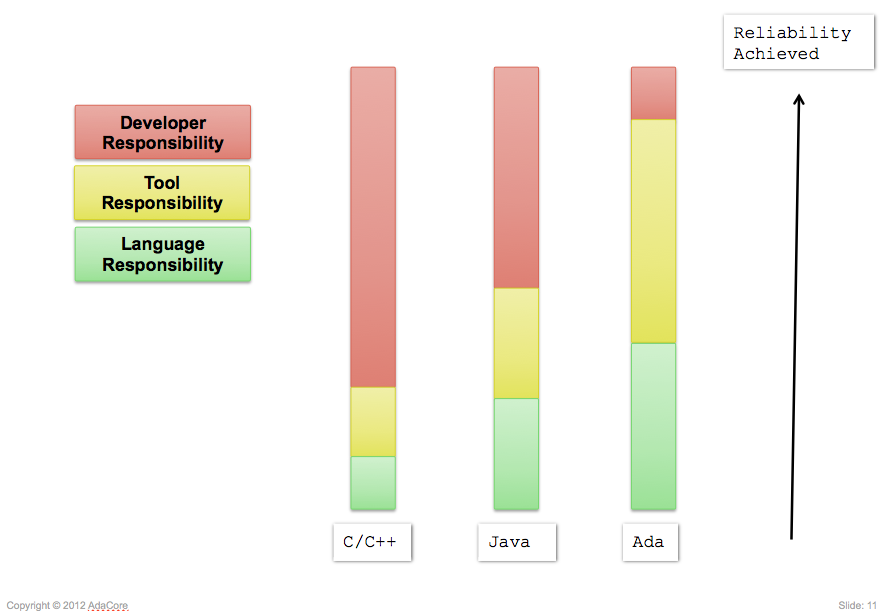
\includegraphics[height=4.5in]{figures/developer_responsibility_in_ada.png}
    	\caption{Developer responsibility in Ada.}
    \end{center}
\end{figure}
%http://www.slideshare.net/AdaCore/ada-2012 (slide 11: dev responsibility)
The most popular IDE for SPARK/Ada is GNAT Programming Studio \footnote{http://libre.adacore.com/tools/gps}.

There is also plugin for Eclipse: GNATbench \footnote{https://www.adacore.com/gnatpro/toolsuite/gnatbench/} created by AdaCore. 
Tools for corectness proving.

\subsection{GNAT Programming Studio}
\label{background:spark:gps}
IDE for SPARK/Ada programs development. Includes proving tools. E.g. Sireum Kiasan (developed by SAnToS lab) or GNAT Prove.


\subsection{Sireum Bakar}
\label{background:spark:sireum}
Overview: symbolic execution, Pilar, Kiasan and Alir \cite{Hari:Thesis}.
Sireum Kiasan \cite{Kiasan:Paper} is a tool, which use symbolic execution for finding possible paths in program.
Plugin for GNAT Programming Studio.
Plugin for Eclipse (but only SPARK 2005).


\subsection{GNAT Prove}
\label{background:spark:gnatprove}
GNATprove \footnote{http://www.open-do.org/projects/hi-lite/gnatprove/} is a formal verification tool for SPARK/Ada programs. It interprets SPARK/Ada annotations exactly like they are interpreted at run time during tests.
% http://docs.adacore.com/spark2014-docs/html/ug/gnatprove.html


\subsection{AUnit}
\label{background:spark:aunit}
Overview
AUnit tutorials \cite{AUnitTutorials:Online}
AUnit Cookbook \cite{AUnitCookbook:Online}



\section{PCA Pump}
\label{background:pcapump}
http://www.santoslab.org/pub/paper/LarsonEtAl13-PCA-Requirements-SEHC-preprint.pdf



\section{AADL/BLESS to SPARK/Ada code generation(maybe translation is better word?)}
\label{background:codegen}
The ultimate goal of long term research, this thesis is part of.
AADLto Ada
BLESS to SPARK contracts + (eventually) behavior


\subsection{Ocarina}
\label{background:codegen:ocarina}
Ocarina \cite{Ocarina:Paper,Ocarina:Paper} generates code from an AADL architecture model to an Ada application running on top of PolyORB framework. In this context, PolyORB acts as both the distribution middleware and execution runtime on all targets supported by PolyORB.
It generate Ada 2005 and C code.
Since mid-2009, Telecom ParisTech is no longer involved in Ocarina, and is developping another AADL toolchain, based on Eclipse, codenamed RAMSES \cite{Ocarina:About:Online}.


\subsection{Ramses}
\label{background:codegen:ramses}
RAMSES is a model transformation framework dedicated to the refinement of AADL models.
% http://www.aadl.info/aadl/downloads/committee/feb2013/presentations/RAMSES_status_2013_06_02_format.pdf
% https://wiki.sei.cmu.edu/aadl/index.php/OSATE_2_on_the_command-line